\chapter{Background}
\label{c:background}
In this chapter we will discuss the background of our system.
The main approch of our system is to improve the traffic light detection using smartphone sensor.
In first part of this chapter we will discuss the inertial sensor of Android and sensor fusion.
Later we will discuss the traffic bulb detection process.

\section{Inertial sensor of smartphone}
\subsection{Accelerometer}
Accelerometer is one of the motion sensor in smartphone.
Smartphone now a days have three axis accelerometer,which can measure acceleration along this three axis and return a vector in the reference frame.
Accelerometer can not measure free fall acceleration rather it measure the forces that are applied to the sensor itself.
For example, when phone is on the table, it will measure acceleration of g, the acceleration due to gravity, because this is proportional to the accelerometer experienced weight.

Figure \ref{f:acc} shows the reference coordination system of accelerometer in Android phone.
The device measures acceleration $a_x$, $a_y$ and $a_z$ along the three axis of android reference frame.
The acceleration $a_z$ points towards the outside of screen face, that is perpendicular to the phone plane.
The acceleration $a_x$ and $a_y$ are along to phone plane.

\begin{figure*}[!ht]
\centering
\subfloat[Accelerator coordination] {\label{f:acc}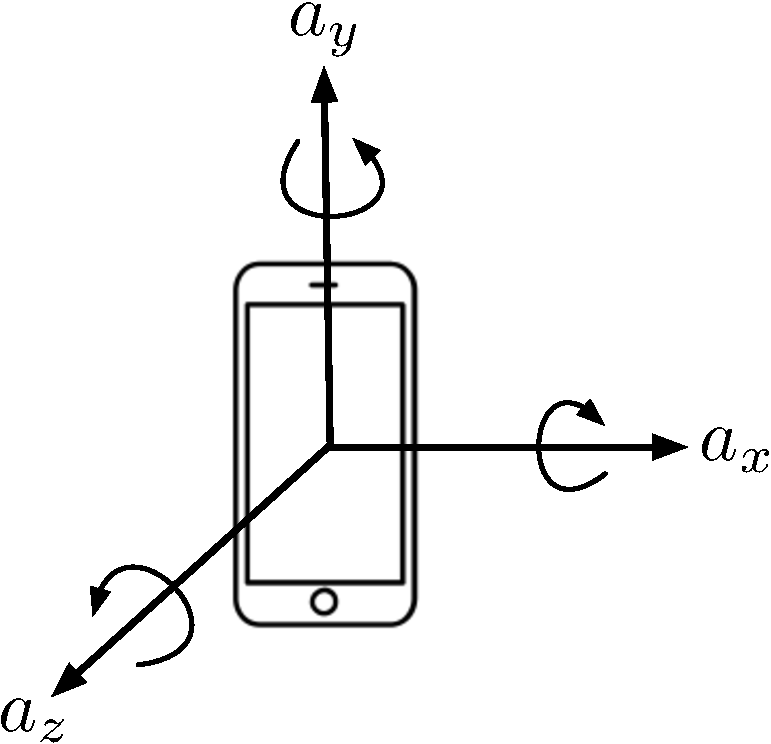
\includegraphics[width=2.5in]{figures/coord_acceleration.pdf}}
\hfill
\subfloat[Gyroscope coordination] {\label{f:gyro}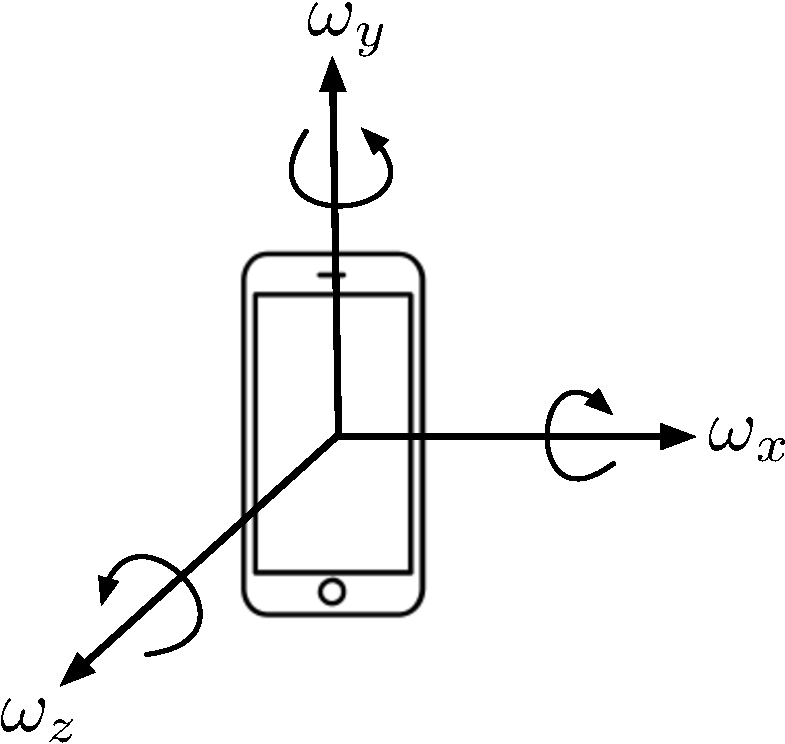
\includegraphics[width=2.5in]{figures/coord_omega.pdf}}

\caption{Smartphone reference coordination system.}
\label{f:coord_dia}
\end{figure*}

\subsection{Gyroscope}
Gyroscope measure the rate of rotation or the angular velocity of rotation along the three axis of smartphone's reference frame.
This is also a motion sensor of smartphone like accelerometer.
These gyroscope use MEMS (micro-electro-mechanical sensing) technology, contain vibrating elements to measure Coriolis effect.
When smartphone rotates, there is a change of direction of vibrating elements because of the Coriolis force.
MEMS gyroscope measure these variation along the three axis to estimate the rate of rotation.
Gyroscope output is quite smooth, and very responsive to small rotations.

Figure \ref{f:gyro} shows the reference coordination system of gyroscope in Android phone.
The device measures rate of rotaion $\omega_x$, $\omega_y$ and $\omega_z$ along the three axis of android reference frame.
The angular velocity of rotation $\omega_z$ points towards the outside of screen face, that is perpendicular to the phone plane, which is the angular velocity of phone's rotaion in X-Y plane.
The rate of rotation $\omega_x$ and $\omega_y$ is along with the phone plane, which is the angular velocity of phone's rotaion in Y-Z plane and Z-X plane respectively.

\subsection{Geomagnetic field sensor}
Geomagnetic field sensor is a position sensor of smartphone.
It helps to determine the device's physical position in the world's reference frame.
Geomagnetic field sensor mesure the change of magnetioc field and estimates the magnetic field at earth's point to find the declination from the true North.
It provides the geomagnetic field strength along the three coordination axis of refernce frame.


\subsection{Orientation}
Each sensor defined in previous section has it's own strength and weakness.
Gyroscope is fast, accurate and reliable.
It is very responsive to small rotation so it can track the change of rotation at every timestamp.
But gyroscope data can not measure gravity.
So with accelerometer it can provide a better rotation or motion of the sensor in application's frame reference.
But to have the position of the device in world's reference frame, we need to fused this data with geomagnetic field sensor.
Another motion sensor in android, rotation vector, use this three sensor data to report the orientation of the device in vector form along the axis of reference frame.

This rotation vector provides the axis of the system and the angle of rotation from these axis.
From this angle and axis data, we can get the orientation of the system in terms of pitch, roll and azimuth.

\begin{figure}
\centering
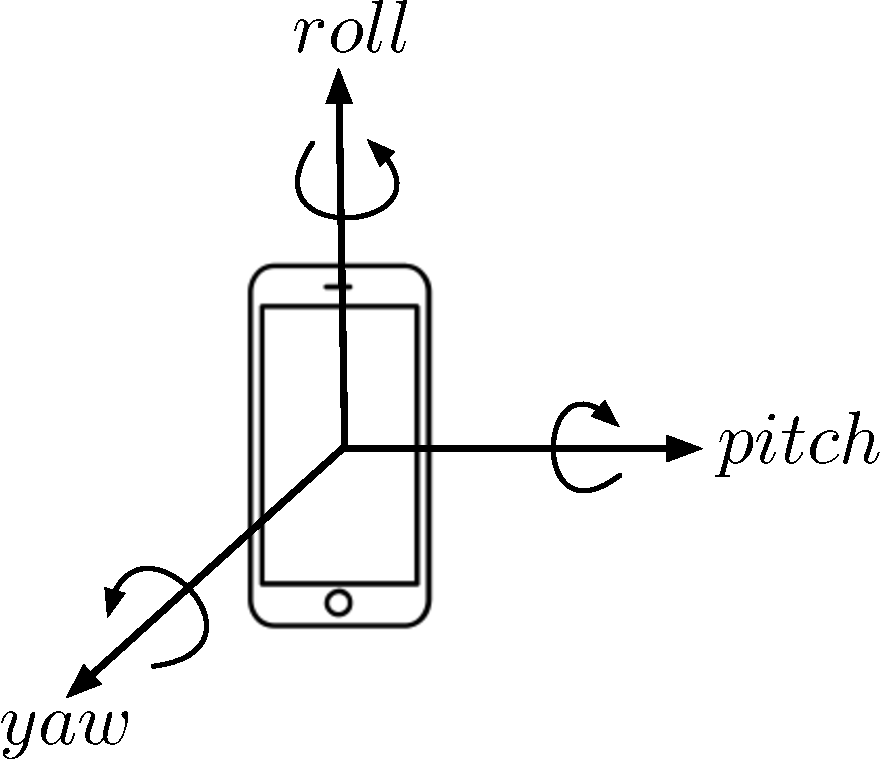
\includegraphics[width=3.8in]{figures/roll_pitch_yaw.pdf}
\caption{Orientation of the smartphone}
\label{f:rpy_dia}
\end{figure}

\ref{f:rpy_dia} shows the orientation of a smartphone about the device's coordination system.
Pitch is the degree of rotation about the X axis.
This is the angle between the plane parallel to device and parallel to the ground.
If device top edge incle to the ground the pitch will be positive and vice versa.
The range of pitch value is -180 degrees to 180 degrees.
Roll is the degree of rotation abot Y axix.
This is the angle between the plane perpendicular to device and perpendicular to ground.
If device's left edge inclenes to the ground roll value is positive.
The range of roll value is -90 degrees to 90 degrees.
Azimuth is the degree of rotation about Z axis.
If the device is faced to the earth's North the azimuth is 0 degree.
Azimuth is 90 degree at earth's East, 180 degree to earth's South and 270 degree to earth's West.

\section {Image Processing}

\subsection{Color Space}
The main two color spaces for processing the color vision are RGB color space and HSV color space.
RGB is a additive color space.
RGB color space describes colors with the amount of red, green and blue color presents on that frame.


\ref{f:rgb} shows the model of RGB space.
It shows that any color of this cube is made of red,blue, and green color.

HSV color space is similar to the way human sees the color.
But RGB defines color in relation to the primary colors.
HSV color space describes color in terms of Hue, Saturation and Value.
It separates the color information from the intensity or the brightness.
Hue is the continuous representation of color type.
In HSV, hue is an angle from 0 to 360 degree. 
But since OpenCv can process data from 0 to 255, so in OpenCv the range is halved.
Every color can be discrimated with the different range of Hue.
Saturation represents the vibracy of the color.
The ranges for saturation is 0 to 255.
The lower saturation meaning gray is present in the color, higher saturation represents primary color.
Value represents brightness of the color.
The range of value is same as saturation, 0 to 255.
Lower value means less bright color, 0 brightness represents black color.

\begin{figure}[htbp]
\begin{minipage}[t]{0.45\linewidth}
    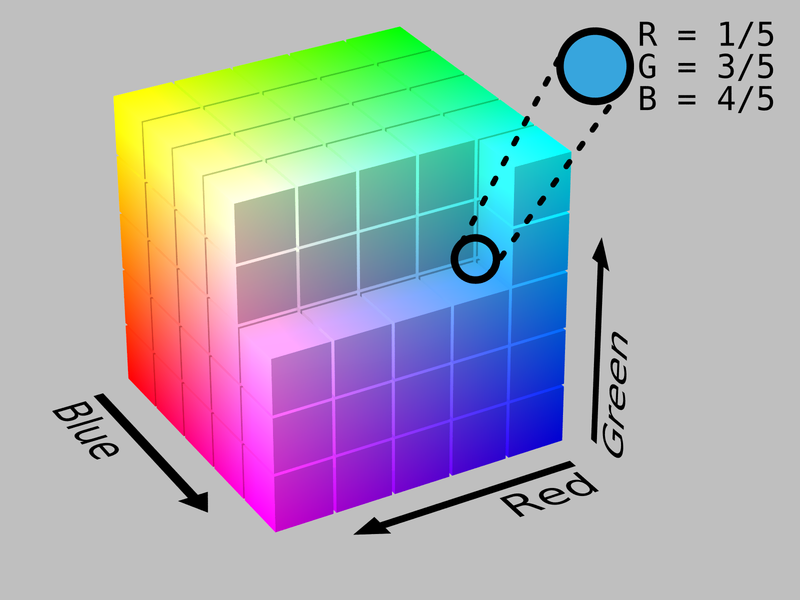
\includegraphics[width=\linewidth]{images/RGB.png}
    \caption{RGB color space}
    \label{f:rgb}
\end{minipage}
    \hfill
\begin{minipage}[t]{0.45\linewidth}
    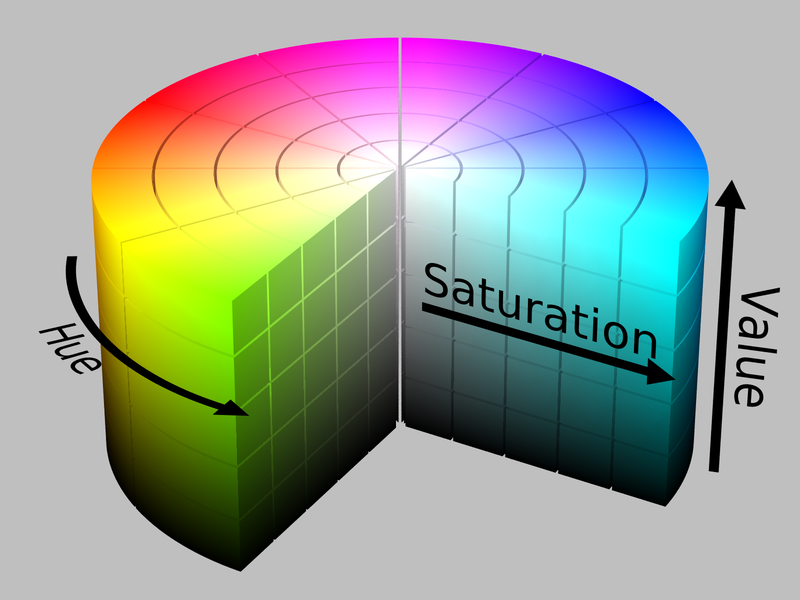
\includegraphics[width=\linewidth]{images/HSV.png}
    \caption{HSV color space}
    \label{f:hsv}
\end{minipage} 
\end{figure}

\ref{f:hsv} shows the cylindrical model of HSV color space.
The Hue is the circular part.
The radious of this circular part represent Saturation and the height is the Value.

\subsection{Hough Circle Transform}
Our system detects the traffic bulb using the hough circle algorithm \cite{houghcir_alg}.
To detect the circle first process is to find the edges in the input image.
The hough circle algotithm uses canny operation for the edge detection.
At every edge pixel, it generates a circle.
An accumulator matrix is created to find the intersection of these circles.
If circle passes through the grid of the accumulator matrix, it increase the coting number of the grid.
The psition of the local maxima of this accumulator matrix provides the corresponding circles centers.







